\title{Warm-Up for May 9th, 2022}
\author{Dr. Jordan Hanson - Whittier College Dept. of Physics and Astronomy}
\date{\today}
\documentclass[12pt]{article}
\usepackage[a4paper, total={18cm, 27cm}]{geometry}
\usepackage{graphicx}
\usepackage{amsmath}
 
\begin{document}
\small
\maketitle
\section{Memory Bank}
\begin{enumerate}
\item Displacement current: $\mathbf{J}_{\rm D} = \epsilon_0 \frac{\partial \mathbf{E}}{\partial t}$
\item Amp\`{e}re's Law: $\nabla \times \mathbf{B} = \mu_0 \mathbf{J} + \mu_0 \epsilon_0 \frac{\partial \mathbf{E}}{\partial t}$
\end{enumerate}

\section{RC Circuits and RL Circuits}

\begin{enumerate}
\item A fat wire, radius $a$, carries a constant current $I$, uniformly distributed over its corss section.  A narrow gap in the wire, of width $w\ll a$, forms a parallel-plate capacitor, as shown in Fig. \ref{fig:1}.  Find the magnetic field in the gap, at a distance $s < a$ from the axis.
\end{enumerate}

\begin{figure}
\centering
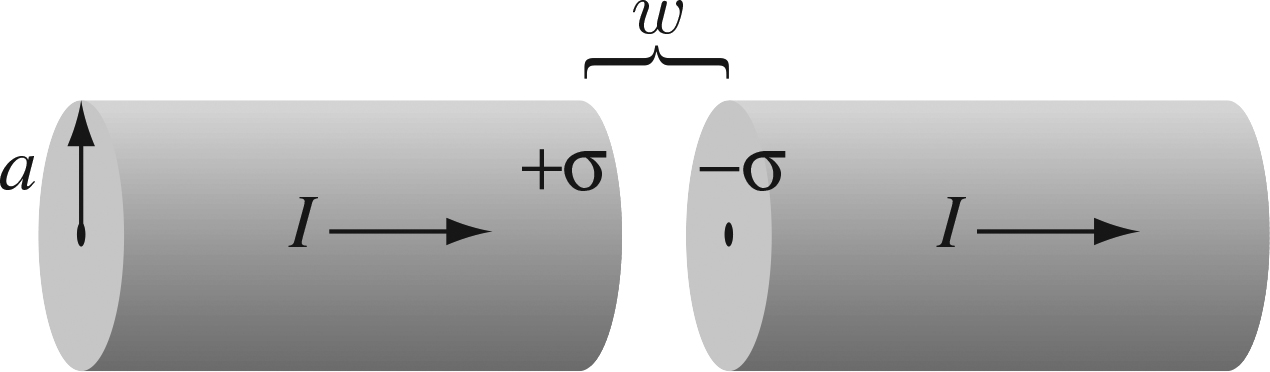
\includegraphics[width=0.5\textwidth]{figures/7_45.jpg}
\caption{\label{fig:1} A small gap of width $w$ in a wire of radius $a$.  The wire carries a current $I$.}
\end{figure}

\end{document}